\documentclass[border=12pt]{standalone}
\usepackage{amsmath, amssymb}
\usepackage{tikz}
\definecolor{ring0}{HTML}{0033CC}
\definecolor{ring1}{HTML}{0066FF}
\definecolor{ring2}{HTML}{0099FF}
\definecolor{ring3}{HTML}{00CCCC}
\definecolor{ring4}{HTML}{00CC66}
\definecolor{ring5}{HTML}{33CC00}
\definecolor{ring6}{HTML}{99CC00}
\definecolor{ring7}{HTML}{CCCC00}
\definecolor{ring8}{HTML}{FF9900}
\definecolor{ring9}{HTML}{FF6600}
\definecolor{ring10}{HTML}{FF3300}
\definecolor{ring11}{HTML}{CC0000}
\definecolor{gap0}{HTML}{E53935}
\definecolor{gap1}{HTML}{1E88E5}
\definecolor{gapfar}{HTML}{CCCCCC}
\begin{document}
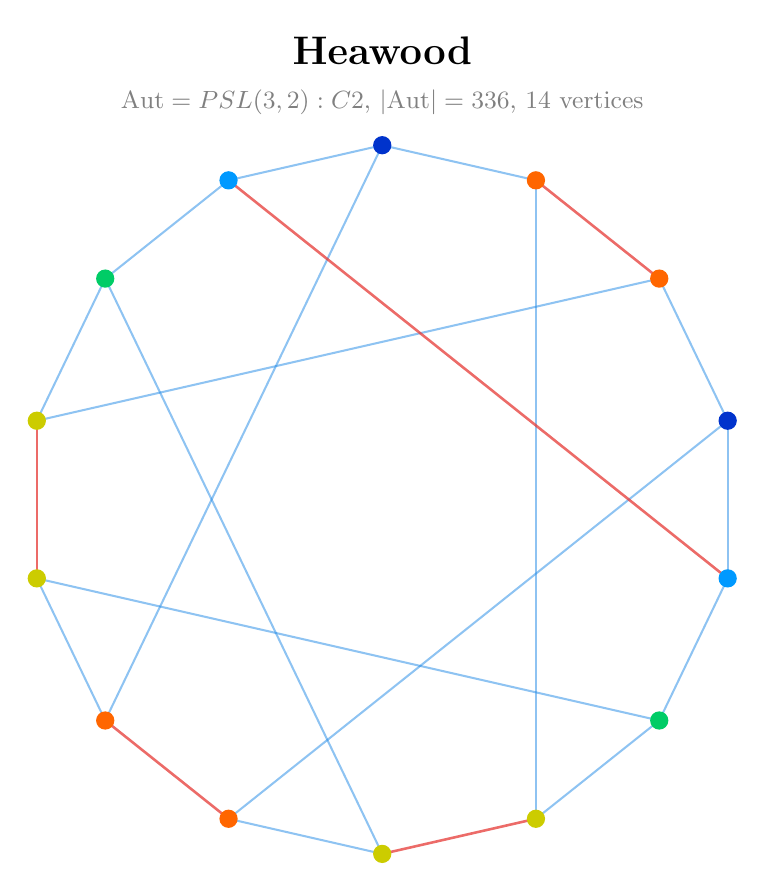
\begin{tikzpicture}
\node[font=\Large\bfseries] at (0, 5.70) {Heawood};
\node[font=\small, text=gray] at (0, 5.05) {$\mathrm{Aut} = PSL(3,2) : C2$, $|\mathrm{Aut}| = 336$, 14 vertices};
\draw[line width=0.74pt, gap1, opacity=0.50] (0.000, 4.500) -- (-1.952, 4.054);
\draw[line width=0.74pt, gap1, opacity=0.50] (0.000, 4.500) -- (-3.518, -2.806);
\draw[line width=0.74pt, gap1, opacity=0.50] (0.000, 4.500) -- (1.952, 4.054);
\draw[line width=0.74pt, gap1, opacity=0.50] (-1.952, 4.054) -- (-3.518, 2.806);
\draw[line width=0.74pt, gap1, opacity=0.50] (-3.518, 2.806) -- (-4.387, 1.001);
\draw[line width=0.74pt, gap1, opacity=0.50] (-3.518, 2.806) -- (-0.000, -4.500);
\draw[line width=0.74pt, gap1, opacity=0.50] (-4.387, 1.001) -- (3.518, 2.806);
\draw[line width=0.74pt, gap1, opacity=0.50] (-4.387, -1.001) -- (-3.518, -2.806);
\draw[line width=0.74pt, gap1, opacity=0.50] (-4.387, -1.001) -- (3.518, -2.806);
\draw[line width=0.74pt, gap1, opacity=0.50] (-1.952, -4.054) -- (-0.000, -4.500);
\draw[line width=0.74pt, gap1, opacity=0.50] (-1.952, -4.054) -- (4.387, 1.001);
\draw[line width=0.74pt, gap1, opacity=0.50] (1.952, -4.054) -- (3.518, -2.806);
\draw[line width=0.74pt, gap1, opacity=0.50] (1.952, -4.054) -- (1.952, 4.054);
\draw[line width=0.74pt, gap1, opacity=0.50] (3.518, -2.806) -- (4.387, -1.001);
\draw[line width=0.74pt, gap1, opacity=0.50] (4.387, -1.001) -- (4.387, 1.001);
\draw[line width=0.74pt, gap1, opacity=0.50] (4.387, 1.001) -- (3.518, 2.806);
\draw[line width=0.93pt, gap0, opacity=0.75] (-1.952, 4.054) -- (4.387, -1.001);
\draw[line width=0.93pt, gap0, opacity=0.75] (-4.387, 1.001) -- (-4.387, -1.001);
\draw[line width=0.93pt, gap0, opacity=0.75] (-3.518, -2.806) -- (-1.952, -4.054);
\draw[line width=0.93pt, gap0, opacity=0.75] (-0.000, -4.500) -- (1.952, -4.054);
\draw[line width=0.93pt, gap0, opacity=0.75] (3.518, 2.806) -- (1.952, 4.054);
\fill[ring0] (0.000, 4.500) circle (3.3pt);
\fill[ring2] (-1.952, 4.054) circle (3.3pt);
\fill[ring4] (-3.518, 2.806) circle (3.3pt);
\fill[ring7] (-4.387, 1.001) circle (3.3pt);
\fill[ring7] (-4.387, -1.001) circle (3.3pt);
\fill[ring9] (-3.518, -2.806) circle (3.3pt);
\fill[ring9] (-1.952, -4.054) circle (3.3pt);
\fill[ring7] (-0.000, -4.500) circle (3.3pt);
\fill[ring7] (1.952, -4.054) circle (3.3pt);
\fill[ring4] (3.518, -2.806) circle (3.3pt);
\fill[ring2] (4.387, -1.001) circle (3.3pt);
\fill[ring0] (4.387, 1.001) circle (3.3pt);
\fill[ring9] (3.518, 2.806) circle (3.3pt);
\fill[ring9] (1.952, 4.054) circle (3.3pt);
\end{tikzpicture}
\end{document}